%
% cre.tex (LateX)
% 
% Objetivo: Capítulo sobre o método CRE do relatório de qualificação de doutorado.
% 
% Versão 1.0
% 
% Site: http://www.dirackslounge.online
% 
% Programador: Rodolfo A. C. Neves (Dirack) 07/10/2019
% 
% Email: rodolfo_profissional@hotmail.com
% 
% Licença: GPL-3.0 <https://www.gnu.org/licenses/gpl-3.0.txt>.

\chapter{EMPILHAMENTO POR ELEMENTO DE REFLEXÃO COMUM (ERC)}

O método do Elemento de Reflexão Comum (ERC) é uma alternativa para os métodos usuais de empilhamento PMC ou
migração para a seção de afastamento nulo. Não requer conhecimento do modelo geral em subsuperfície, apenas
o conhecimento da velocidade próxima a superfície é necessário a priori.
O método ERC é baseado somente em considerações cinemáticas em 2D e não é
um processo que preserva as amplitudes.
A principal e provavelmente mais importante vantagem do método ERC em comparação com o empilhamento PMC convencional
é que este proporciona, além da seção empilhada, parâmetros importantes para a construção do macromodelo de 
velocidades que pode inclusive variar lateralmente \cite{cre}.

As principais características do método ERC:
(a) A construção da seção de afastamento nulo a partir de um conjunto de seções de afastamento constante
com apenas uma estimativa da velocidade próxima da superfície.
(b) A determinação dos parâmetros $(R_{NIP},\beta_0)$ para as reflexões de afastamento nulo na seção empilhada.
Estes atributos podem ser utilizados com técnicas de inversão para estimar o macromodelo de velocidades.

Os parâmetros $R_{NIP}$ e $\beta_0$ 
são atributos específicos de uma frente de onda hipotética atribuídos a cada evento de reflexão
primária de afastamento nulo: O raio de curvatura $R_{NIP}$ e o ângulo de emergência $\beta_0$. Esta onda hipotética é
a onda NIP \cite{hubral}.

A idéia principal do método ERC é, usando a fórmula do tempo de trânsito ERC, no modelo auxiliar, dado um intervalo
de busca para os parâmetros $R_{NIP}$ e $\beta_0$, encontrar a frente de onda NIP que melhor se ajusta aos dados.
Este processo é semelhante a análise sobretempo normal convencional, todavia enquanto esta análise é feita no
domínio PMC, o método ERC é feito no domínio ERC construído durante o processo, o parâmetro otimizado $R_{NIP}$,$\beta_0$
é especificado a partir da análise de coerência nos dados \cite{cre}.


As coordenadas das curvas ERC, mesmo sem o conhecimento da curvatura do refletor em subsuperfície, são definidas
a partir dos parâmetros $R_{NIP}$ e $\beta_0$, obtidos através de algum processo de orimização, 
para cada PMC central $m_0$ na seção de afastamento nulo. A equação que descreve a trajetória ERC no plano $m,h$:

\begin{equation}
 \label{eq:4.65}
 x_m= x_0 + \frac{1}{2\alpha} (1-\sqrt{1+4\alpha^2h^2})
\end{equation}


Onde $\alpha$ é um parâmetro de assimetria que desenpenha um papel importante na seleção de pares fonte-receptor para os quais
o correspondente raio de reflexão refletem no mesmo ponto sobre o refletor \cite{tygel}. É dado por:

\begin{equation}
\label{eq:4.67}
 \alpha=\frac{\sin{\beta_0}}{R_{NIP}}
\end{equation}

Os traços sísmicos com as coordenadas $m,h$ dadas pela Equação \ref{eq:4.65} formam uma família ERC.
O método ERC também possui uma aproximação de tempo de trânsito para
as reflexões \cite{cre}:

\begin{multline}
\label{eq:4.66}
t(m,h)=(\tau_0-\frac{2R_{NIP}}{v_0})+\frac{R_{NIP}}{v_0}\sqrt{1-2\alpha(m-m_0+h)+\frac{(m-m_0+h)^2}{R_{NIP}^2}} \\
+\frac{R_{NIP}}{v_0}\sqrt{1-2\alpha(m-m_0-h)+\frac{(m-m_0-h)^2}{R_{NIP}^2}}
\end{multline}

\begin{figure}[H]
\caption{Representação esquemática de um arranjo ERC para um refletor circular de raio $R$ e profundidade
mínima $D$: A família ERC é formada pelos pares $s_i$-$r_i$ (fonte-receptor) que possuem o mesmo ponto de
reflexão em subsuperfície ($NIP$). A família ERC pode ser entendida a partir de uma fonte pontual explosiva
no ponto $NIP$, que ao ser ativada forma uma frente de onda $NIP$ que atinge a superfície em um PMC central 
$m_0$ com raio de curvatura $R_{NIP}$ e ângulo de incidência $\beta_0$.}
\begin{center}
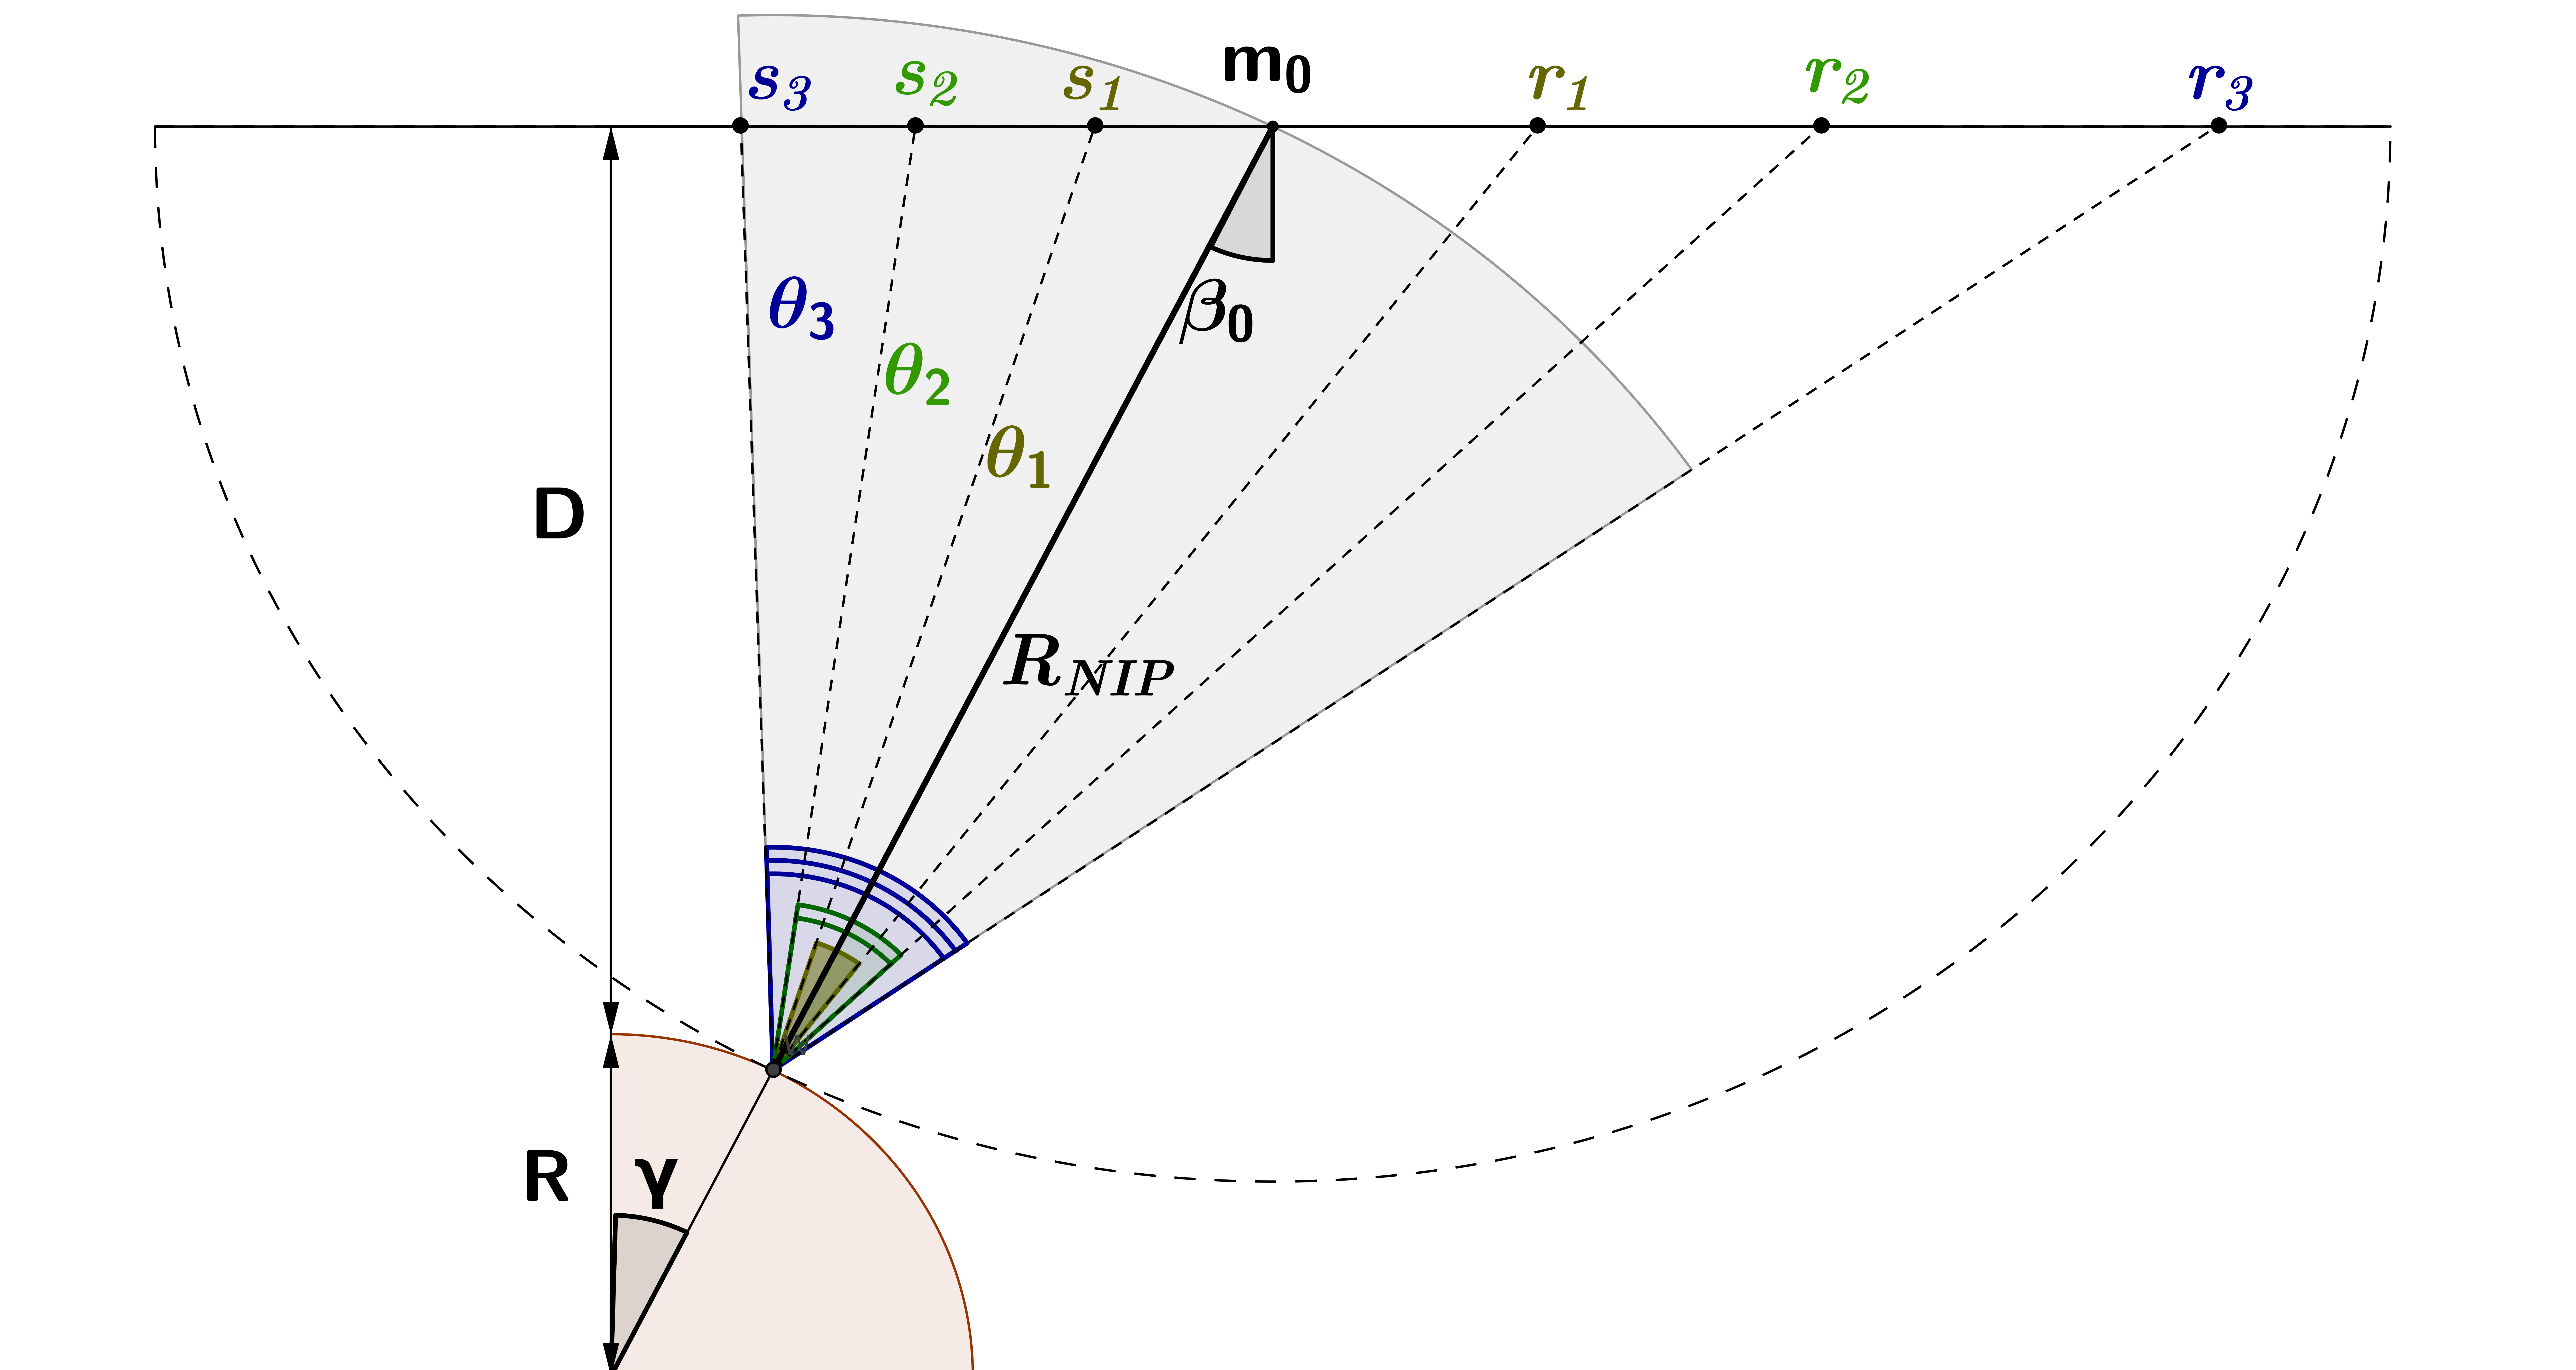
\includegraphics[scale=0.3]{images/cre.png}
\vspace{-0.3cm}
\end{center}
\begin{center}
 Fonte: Do Autor.
\end{center}
\label{fig:4.1}
\end{figure}

O principal desvantagem do método ERC é que as coordenadas de fontes e receptores são distribuídas assimetricamente em tal 
arranjo: Na Figura \ref{fig:4.1} representamos um arranjo ERC em um modelo do refletor circular 
em um meio com velocidade constante $v$.
Todos os raios de reflexão que saem das fontes $s_i$ e chegam aos receptores $r_i$ 
possuem o mesmo ponto de reflexão sobre o refletor.
Porém, a curvatura do refletor estabelece uma distribuição assimétrica dos pares fonte e receptor no domínio do afastamento
e na distância em relação ao PMC central $m_0$.

A Figura \ref{fig:4.2} mostra as coordenadas $m,h$ de várias curvas ERC hipotéticas com $\alpha$ dado pela Equação \ref{eq:4.66}.
As curvas ERC intersectam as seções de afastamento constante (linhas horizontais) e as seções de ponto médio comum 
(linhas verticais), não sendo posível construir uma malha regular para amostrar tais curvas.
A única distribuição que pode ser amostrada regularmente no plano $m,h$ ocorre quando $\alpha=0$, que corresponderá
a família de ponto médio comum de um dado $m_0$, uma linha vertical no plano (em roxo).

\begin{figure}[htb]
\caption{Representação esquemática das coordenadas de várias trajetórias ERC sobre o plano PMC $m$ x meio afastamento
$h$. As linhas do grid representam as seções de afastamento constante (linhas horizontais) e seções PMC (linhas verticais).
Estas trajetórias foram construídas variando $\beta_0$, $R_{NIP}$ e $\alpha$  na Equação \ref{eq:4.65}. Quando
$\alpha=0$ a trajetória ERC será a trajetória de uma família PMC para um PMC $m_0$.}
\begin{center}
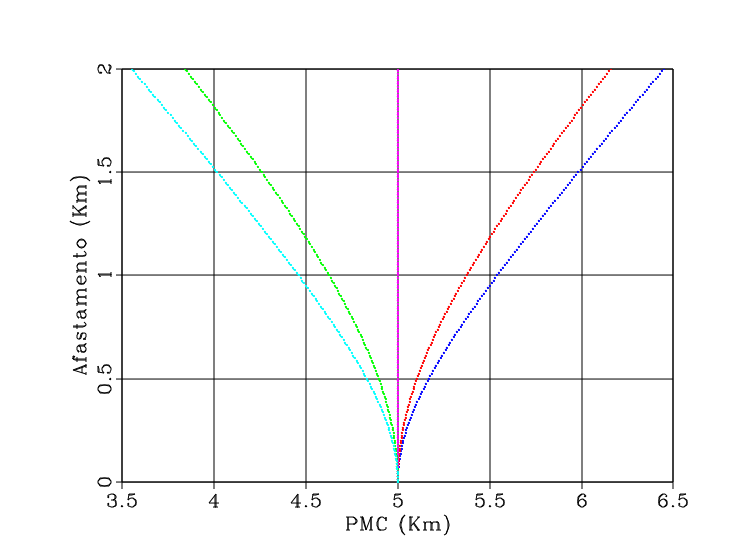
\includegraphics[scale=0.5]{images/creCoord.png}
\vspace{-0.3cm}
\end{center}
\begin{center}
 Fonte: Do Autor.
\end{center}
\label{fig:4.2}
\end{figure}

Portanto, o método ERC é dependente de alguma estratégia de interpolação para os traços sísmicos sobre a trajetória ERC.
E para a obtenção da família ERC, necessita dos parâmetros $R_{NIP}$ e $\beta_0$ no calculo da aproximação da curva de tempo
de trânsito ERC. Estes parâmetros serão utilizada no empilhamento para a obtenção da seção empilhada ERC.
